\section{Systemarchitektur}

Bei der Implementierungsarbeit zum Projekt wurde auf eine schlanke, modular gekapselte und erweiterbare Systemarchitektur zur Erfassung, Verarbeitung und Analyse der Daten aus verschiedenen Musikinformationsquellen geachtet. Aufgrund der einfach zu handhabenden prototypischen Entwicklung und gute Unterst�tzung durch Open Source Bibliotheken von Drittherstellern wurde Java innerhalb Eclipse IDE als Zielsprache gew�hlt. 


\subsection{MIR Framework}

Der Hauptanteil der Entwicklung fokusiert sich auf die Datenerfassung und Aufbereitung verschiedenster deskriptiver und numerischer Eigenschaften aus unterschiedlichsten Datenquellen zu einer K�nstler Entit�t \texttt{MirArtist}. Abb.~\ref{fig:systemarchitecture} zeigt die Grundz�ge der Systemarchitektur, die in f�nf Ebenen gegliedert ist. Neben der Datenerfassung, Informationsextraktion und �hnlichkeitsberechung wurde auch Wert auf die visuelle Aufbereitung der Ergebnisse in Form von Charts, Netzwerkgraphen und Clustern gelegt. Drei heterogene \textbf{Datenquellen} wurden zur Erfassung von k�nstlerbezogenen Features herangezogen:
\begin{figure}[ht]
	\centering
	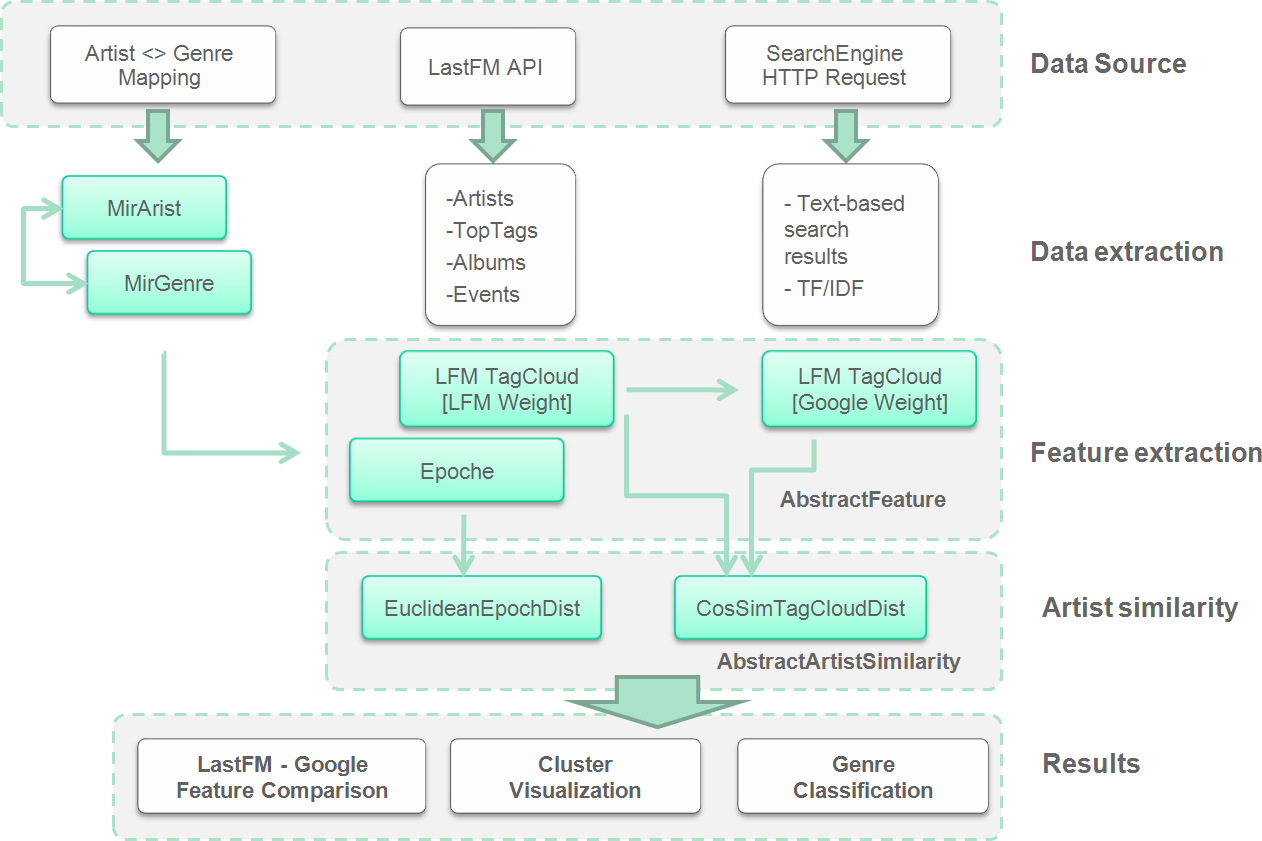
\includegraphics[width=0.8\textwidth]{images/systemarchitecture.png} % \textwidth
	\caption{System Architektur des im Rahmen des Projekts entwickelten MIR Frameworks}
	\label{fig:systemarchitecture}
\end{figure} 


\begin{itemize}
	\item \textbf{Artist-Genre Mapping:} Das Textfile-basierte Mapping von 224 K�nstlern (je 11 in 14 Genres) war Teil der �bungsbeschreibung.
	\item \textbf{LastFM API:} Die API zu dem Musikportal LastFM war die Hauptquelle zur Erfassung vieler k�nstlerbezogener Daten wie etwa TopTags, Album Release Dates, Auftrittsorte (Events und Venues). F�r die SOAP-basierte Schnittstelle stand eine Java-Bibliothek zur Verf�gung. Diese wurde modifiziert um neben den Top Tags auch die Tag-Gewichte f�r akkurater �hnlichkeitsberechungen erfassen zu k�nnen.
	\item \textbf{Search Engine Queries:} Um einen Vergleich zwischen den �hnlichkeiten der Community-basierten LastFM Platform und einer nicht benutzergetrieben Datenquelle herstellen zu k�nnen, wurde ein dem CoMIRVA Framework\footnote{CoMIRVA Framework - http://www.cp.jku.at/comirva/} angelehnter \texttt{UrlRetriever} f�r Suchmaschinenabfragen implementiert, der auf Basis der ersten $N$ Linkresultate in Google ein \texttt{UrlDownloader} zum Download der Pages anregt.
\end{itemize}

Auf Ebene der \textbf{Featureextraktion} wurde eine Basisklasse \texttt{Feature} eingef�hrt, die die Heterogenit�t der k�nstlerbezogenen Eigenschaften wie Genrezugeh�rigkeit, listenbasierter Tag-Wolken und Schaffensperiode aus den Grunddaten extrahiert. Dese Features k�nnen nicht direkt instanziert werden, sondern werden durch eine \texttt{FeatureFactory}, die den Zugriff zum Datenlayer kapselt, generiert. Jedes abstrakte Feature kann anschlie�end unter einem gemeinsamen Interface beim zugeh�rigen Artist registiert werden. 

F�r die \textbf{�hnlichkeitsberechung }wurde ebenfalls eine \texttt{AbstractSimilarityMeasure} Basisklasse definiert, die die Ableitung von konkreten Klassen zur Berechung von symmetrischen �hnlichkeitsmatrizen zwischen $NxN$ K�nstlern erlaubt. Jedes �hnlichkeitsma� wei� �ber den internen Aufbau eines konkreten Features Bescheid und kann auf dieses unter Zuhilfenahme einer eindeutigen FeatureID darauf zugreifen falls das Feature zuvor berechnet und registriert wurde. Abb.\ref{fig:flowchart} zeigt das Flussdiagramm einer modularen Featureaggregation innerhalb eines einzelnen K�nstlern. Sofern f�r jedes Feature oder eine Sammmlung an Features ein entsprechendes SimilarityMeasure implementiert wurde kann ein numerische �hnlichkeitsmatrix als normiertes \textbf{Resultat} f�r die textbasierte Interpretation, eine Visualisierung aber auch einen Genre-Klassifikationversuch herangezogen werden. 

\begin{figure}[ht]
	\centering
	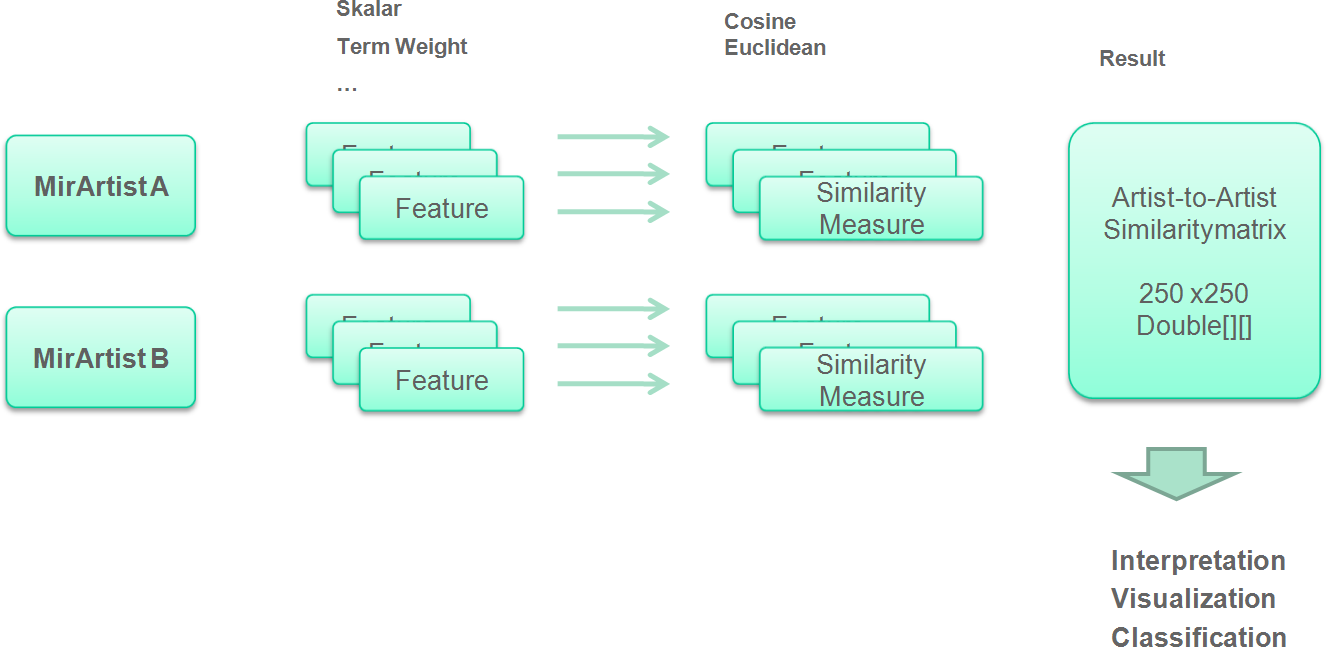
\includegraphics[width=0.7\textwidth]{images/flowchart.png} % \textwidth
	\caption{Informationsextraktion - \texttt{MirArtist} vereinheitlichte Datenaggregation}
	\label{fig:flowchart}
\end{figure} 


\subsection{Metriken und Tools}

Im Zuge des Projekts wurden unter Verwendung einiger stark modifizierter Fremdklassen �ber 4000 LoC in 60 Klassen (11 Packages) entwickelt. Abb.~\ref{fig:mainclasses} zeigt in einem Abh�ngigkeitsgrafen die Hauptklassen rund um die \texttt{MirArtist}-Entit�t. Die flexible Architektur und gute Kapselung der Teilaufgaben erm�glichte ein rasches Prototyping und gro�e Wiederverwendbarkeit vor allem des Feature Registrierungsmechanismusses und der abtrakten Klassen zur �hnlichkeitsberechung. Die Entwicklungzeit jedes weiteren Features konnte damit drastisch gesenkt werden und erm�glichte eine umfangeiche Analyse zur Dateninterpretation, Vergleichsberechung und zu anschlie�enden Visualisierungs- und Klassifikationsversuchen.

\begin{figure}[ht]
	\centering
	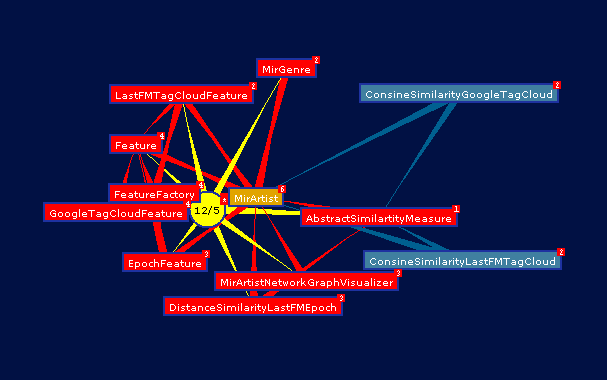
\includegraphics[width=0.6\textwidth]{images/classes.png} % \textwidth
	\caption{Visualisierter Abh�ngigkeitsgraph der Hauptklassen rund um \texttt{MirArtist}.}
	\label{fig:mainclasses}
\end{figure} 



